\section{Sensitivity to Deterministic Parameter Choice}
\label{sec:AngleResults}

At this point in the work, it has been shown how the $\Omega$-methods
behave in problems with differing geometries and materials.
However, each of these problems was run with the same deterministic calculation
parameters. While the angular flux may have differed in these problems due to
the material or geometric configuration, it did not vary due to deterministic
solver choices. Some deterministic solver choices will change the angular
fluxes used to calculate the $\Omega$-flux. Consequently, this may affect the
behavior of the $\Omega$-methods. This section will
explore the effects of deterministic solver
choices on the $\Omega$-methods' performance.

Section \ref{sec:CharResults} showed that the $\Omega$-methods have a strong
weakness to ``thin'' materials, as CADIS and FW-CADIS do. This is because the
importance of a particle may vary several orders of magnitude over a mean free
path of travel distance. At a collision, the particle then requires
several orders of
magnitude of sampling events. This was confirmed by
running the steel beam problem with air and concrete in the geometric location
of the steel beam. In
the ``thin'' material air version, CADIS-$\Omega$ performs poorer than CADIS,
conversely to the original steel problem.
The characterization problem results also showed that
the incorporation of the $\Omega$-flux into a problem with materials with
strongly different moderating properties, the steel plate in concrete, showed
strong improvement when compared to both CADIS and nonbiased Monte Carlo.

Due to the better performance of CADIS-$\Omega$ than CADIS
in the problem with a steel beam in concrete, this is the problem that will be
used to characterize the $\Omega$-methods' sensitivity to deterministic
parameter choice.
In this section, the effect of deterministic solver choices on the
performance of the $\Omega$ methods will be investigated. In particular, we are
interested in how parameters that influence the angular flux will affect the
performance of the $\Omega$-methods. By using the same problem
with differing solver options, the effect of solver options can be isolated from
the material and geometric effects. By doing so, we seek to determine how
resilient the $\Omega$-methods may be by using low-fidelity solver options, how
different the sensitivity of the $\Omega$-methods are to solution quality when
compared to CADIS, and how varying angular parameters may speed up or slow down
the time to a desired solution. By quantifying these effects, we can determine
the best parameter selection for the $\Omega$-methods for this type of problem.

\subsection{Parametric Study Description}
\label{subsec:parstudy}

The angle sensitivity parametric study will cover the subset of computational parameters
that are most likely to influence the $\Omega$ method's solution. Because the
$\Omega$-flux is calculated from an angle integration of the forward and adjoint
flux, calculation parameters that are most likely to influence the angular flux
solution are the variables that were perturbed.
The two parameters that will be studied
are the quadrature order and the P$_N$ order.

The quadrature used in a deterministic solution is used do discretize the
problem in angle. Quadrature options are split into two separate selections: the
quadrature set or type, and the quadrature order. Because the $\Omega$-methods
require rotational symmetry, only quadrature sets that have rotational
symmetry (generally these are triangular quadrature sets)
can be used with the $\Omega$-methods. In ADVANTG/Denovo, the triangular
quadrature sets are: linear-discontinuous finite element, level-symmetric, and
quadruple range. As discussed previously, quadruple range is selected as the
ADVANTG default because it has good properties and guarantees positivity in the
flux. Different quadrature sets have separate
properties and are a realm of study unto their own. Thus, we will vary only
quadrature order and not quadrature type in this sensitivity study.

Quadrature orders specify
how fine of a resolution the quadrature set will be. As quadrature order
increases, the size of the angular flux matrices will increase. We expect to
observe much slower deterministic recorded times for high quadrature orders
because of the I/O demand to read and write these values. Recall that the ADVANTG
default quadrature order is 10. The quadrature orders used for the sensitivity
study aimed to choose orders surrounding this value. This resulted in quadrature
orders 5, 7, 10, 12, 15, 17, and 20 being chosen for variations in this
parameter.

The P$_N$ order determines the fidelity of the scattering expansion. The
availability of P$_N$ orders is dependent on the cross section dataset. For the
27G19N cross section library, the P$_N$ order extends to 5. As a result,
P$_N$ orders of 1, 3, and 5 are chosen for variations in this parameter.

While the P$_N$ order
does affect angular information in the problem, it will not change the size of
the angular flux matrices. As a result, deterministic runtimes between
differing P$_N$ orders
may vary, but not as significantly as they will in differing quadrature orders
due to the lack of change in I/O demands as P$_N$ order changes.

Other deterministic parameters may influence the variance reduction parameters
calculated by the $\Omega$ methods.
The spatial discretization, while not a primary factor influencing
the angular flux, still may affect the $\Omega$-methods' performance.
A finer energy group structure may also influence the $\Omega$-method solution.
Finer energy groups will more effectively reflect resonance regions in
scattering and absorption. Scattering effects in certain energy regions will
have angular dependence and, thus, may be a stronger effect on the angular flux
than a coarser energy discretization. Because these particular solution effects
do not directly influence the angular flux, they will not be included
in the angular sensitivity parametric study. This is because the effects on the
angular flux will be hard to isolate from other factors and conclusions drawn
from them will be harder to make.

% Add to conclusion future work.
%However, a study extending to include the
%energy group structure, the spatial discretization, and the quadrature type
%certainly could be an area of future work.

Several factors in the deterministic calculation should not have a strong effect
on the angular flux distribution. These include the spatial solver, the
convergence criteria for the solvers, and the within group solver types.
Because these factors should not influence the angular flux any more than any
other part of the solution, they will not be included in this parametric study.

\subsection{Quadrature Order}
\label{subsec:quadorder}

Table \ref{tab:quad_foms} contains the FOM results for each of the quadrature
orders run in the parametric study. The results are grouped by the relative
error choices so the trend in each in relation to the quadrature order is more
observable. There are many notable observations that one can gather from this
table.

In the tally average relative error subsection of the table, we can see two strong
dips in the FOM in CADIS at S$_N$ orders 5 and 10, and a dip in CADIS-$\Omega$
at S$_N$ order 12. These dips are much larger relatively than in the maximum or
minimum relative errors subsections of the table. This indicates that for these
particular quadrature orders, overall fewer particles contribute to the
detector response across all groups. We can also see that for CADIS-$\Omega$
quadrature orders 10, 15 and 17 all have a similar FOM for the tally average
relative error using the Monte Carlo runtime. However, the FOMS for the same
quadratures decrease more significantly when using T$_{hybrid}$ to calculate the
FOM. This indicates that the increase in deterministic runtime for increasing
quadrature order is not offset by the decrease in calculation time for the Monte
Carlo with a higher fidelity solution. This effect is also stronger in
CADIS-$\Omega$ than it is in standard CADIS, meaning that increasing quadrature
order in CADIS-$\Omega$ more strongly negatively effects the tally average FOM
than CADIS.

The maximum relative error datapoints also have several notable
datapoints. For CADIS, the dips in FOM are still visible for S$_N$ orders 5 and
7, but they

\begin{table}[h!]
  \centering
  \begin{tabular}{lc|ccccc}
\toprule
{} & {} & \multicolumn{2}{c}{CADIS}  & \multicolumn{2}{c}{CADIS-$\Omega$}  & analog \\
{} &  S$_N$ order &     MC  &   MC$_{hybrid}$ & MC & MC$_{hybrid}$ &  MC \\
\midrule
\multirow{7}{*}{tally avg} &  S$_N$ 5 &        683 &       677 &   1.81e+03 &
1.79e+03 &  \multirow{7}{*}{1.39} \\
      {}     &  S$_N$ 7 &   2.55e+03 &  2.53e+03 &   2.46e+03 &     2.45e+03 &    {}   \\
      {}     & S$_N$ 10 &        669 &       659 &   2.96e+03 &     2.93e+03 &    {}   \\
      {}     & S$_N$ 12 &   2.46e+03 &  2.41e+03 &        187 &          183 &    {}   \\
      {}     & S$_N$ 15 &   2.48e+03 &  2.42e+03 &   2.98e+03 &     2.92e+03 &    {}   \\
      {}     & S$_N$ 17 &   2.47e+03 &  2.39e+03 &   2.96e+03 &     2.88e+03 &    {}   \\
      {}     & S$_N$ 20 &   2.46e+03 &  2.35e+03 &   1.89e+03 &     1.81e+03 &    {}   \\
\midrule
\multirow{7}{*}{max RE}  &  S$_N$ 5 &       4.89 &      4.85 &       2.86 &
2.84 &  \multirow{7}{*}{0.0448} \\
      {}     &  S$_N$ 7 &       7.71 &      7.64 &       4.35 &         4.32 &    {}   \\
      {}     & S$_N$ 10 &       3.74 &      3.69 &       6.71 &         6.64 &    {}   \\
      {}     & S$_N$ 12 &       14.3 &      14.1 &      0.764 &        0.748 &    {}   \\
      {}     & S$_N$ 15 &       14.7 &      14.3 &       3.87 &         3.79 &    {}   \\
      {}     & S$_N$ 17 &       14.8 &      14.4 &       7.98 &         7.78 &    {}   \\
      {}     & S$_N$ 20 &       14.1 &      13.5 &       6.09 &         5.85 &    {}   \\
\midrule
\multirow{7}{*}{min RE}  &  S$_N$ 5 &   1.14e+03 &  1.13e+03 &   1.09e+03 &     1.09e+03 &      -- \\
      {}     &  S$_N$ 7 &   1.37e+03 &  1.36e+03 &   1.26e+03 &     1.25e+03 &      -- \\
      {}     & S$_N$ 10 &   1.43e+03 &  1.41e+03 &   1.32e+03 &      1.3e+03 &      -- \\
      {}     & S$_N$ 12 &   1.46e+03 &  1.43e+03 &   1.33e+03 &      1.3e+03 &      -- \\
      {}     & S$_N$ 15 &   1.47e+03 &  1.43e+03 &   1.32e+03 &      1.3e+03 &      -- \\
      {}     & S$_N$ 17 &   1.46e+03 &  1.42e+03 &   1.31e+03 &     1.28e+03 &      -- \\
      {}     & S$_N$ 20 &   1.46e+03 &  1.39e+03 &   1.31e+03 &     1.26e+03 &      -- \\
\midrule
\multirow{7}{*}{Time (mins)}  &  S$_N$ 5 &        302 &       305 &   1.13e+03 &
1.14e+03 &    \multirow{7}{*}{22.3} \\
      {}     &  S$_N$ 7 &        324 &       327 &   1.62e+03 &     1.63e+03 &    {}   \\
      {}     & S$_N$ 10 &        414 &       420 &   2.11e+03 &     2.14e+03 &    {}   \\
      {}     & S$_N$ 12 &        406 &       414 &   2.09e+03 &     2.14e+03 &    {}   \\
      {}     & S$_N$ 15 &        404 &       413 &    2.1e+03 &     2.14e+03 &    {}   \\
      {}     & S$_N$ 17 &        405 &       418 &   2.11e+03 &     2.17e+03 &    {}   \\
      {}     & S$_N$ 20 &        406 &       425 &   2.12e+03 &     2.21e+03 &    {}   \\
\bottomrule
\end{tabular}

  \caption[Figure of Merit results for steel beam embedded in concrete, with
  variations in quadrature order.]{Figure of Merit results for steel beam embedded in concrete, with
  variations in quadrature order. Subdivisions of the table indicate
calculations of the FOM using different relative errors. The analog case has a
single value for each relative error as it is not dependent on changes in
deterministic calculation parameters.}
  \label{tab:quad_foms}
\end{table}

In the minimum relative error subsection of the Table \ref{tab:quad_foms}
the CADIS behavior is
much more well-behaved than it is for the preceding two subsections of the
table. There are no dips in the FOM value, so the lowest relative error will
consistently get better with increasing quadrature order. A slight shift
occurs for quadrature orders 17 and 20, which indicates that increasing
quadrature fidelity does not help improve the FOM past S$_N$ order 15. Similar
behavior is observable for CADIS-$\Omega$ in the minimum relative error
subsection of the table. CADIS-$\Omega$ consistently has a lower-valued FOM
between ~5\%-10\% for all quadrature orders. A turnover occurs in the CADIS-$\Omega$
FOMs at a lower quadrature order, meaning that CADIS-$\Omega$ does not benefit
from increasing S$_N$ order as much as CADIS.

This table shows that for the FOM using the tally average relative error,
CADIS-$\Omega$ outperforms CADIS for most quadrature orders (with excpetions
being S$_N$ orders 7 and 12). It also shows that CADIS-$\Omega$

\begin{figure}[htb!]
  \centering
  \begin{subfigure}[t]{\textwidth}
    \centering
    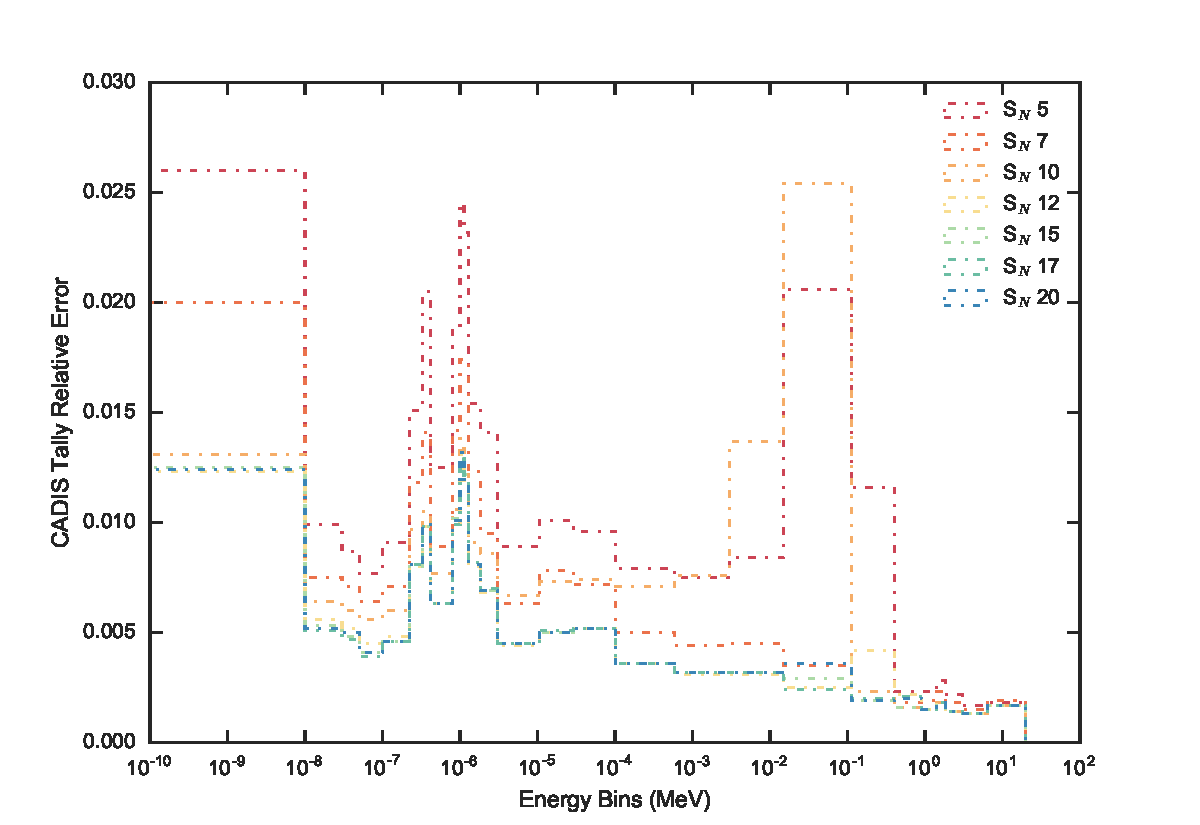
\includegraphics[width=\linewidth]{./chapters/characterization_probs/figures/angle/prob_1/err_quad_cadis.pdf}
    \caption{Relative errors of CADIS results for differing S$_N$ orders.}
    \label{fig:sn_cad_err}
  \end{subfigure}
\end{figure}
\begin{figure}[htb!]\ContinuedFloat
  \centering
  \begin{subfigure}[t]{\textwidth}
    \centering
    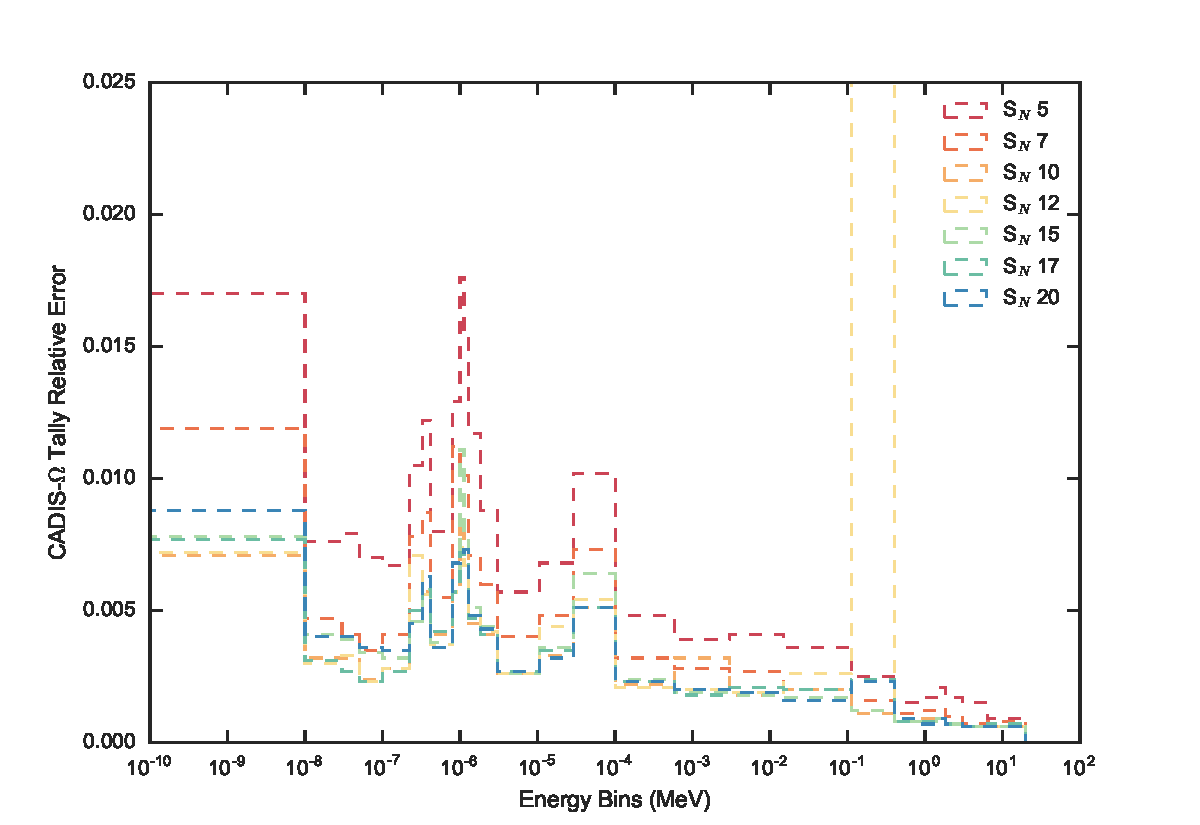
\includegraphics[width=\linewidth]{./chapters/characterization_probs/figures/angle/prob_1/err_quad_cadisangle.pdf}
    \caption{Relative errors of CADIS-$\Omega$ results for differing S$_N$
    orders.}
    \label{fig:sn_cadangle_err}
  \end{subfigure}
  \caption[Relative error results for CADIS and CADIS-$\Omega$ for different
  quadrature orders for the problem with a steel beam in concrete.]
  {Relative error results for CADIS (Figure \ref{fig:sn_cad_err})
  and CADIS-$\Omega$ (Figure \ref{fig:sn_cadangle_err}) for different
  quadrature orders for the problem with a steel beam in concrete.}
  \label{fig:sn_errs}
\end{figure}

Figures \ref{fig:sn_cad_err} and \ref{fig:sn_cadangle_err} show the relative
errors for all tally bins for each quadrature order run of the problem with the
steel beam in concrete. Unlike Table \ref{tab:quad_foms}, these plots show the
overall behavior of the tally results as a function of changing quadrature
order.

\begin{figure}[h!]
  \centering
  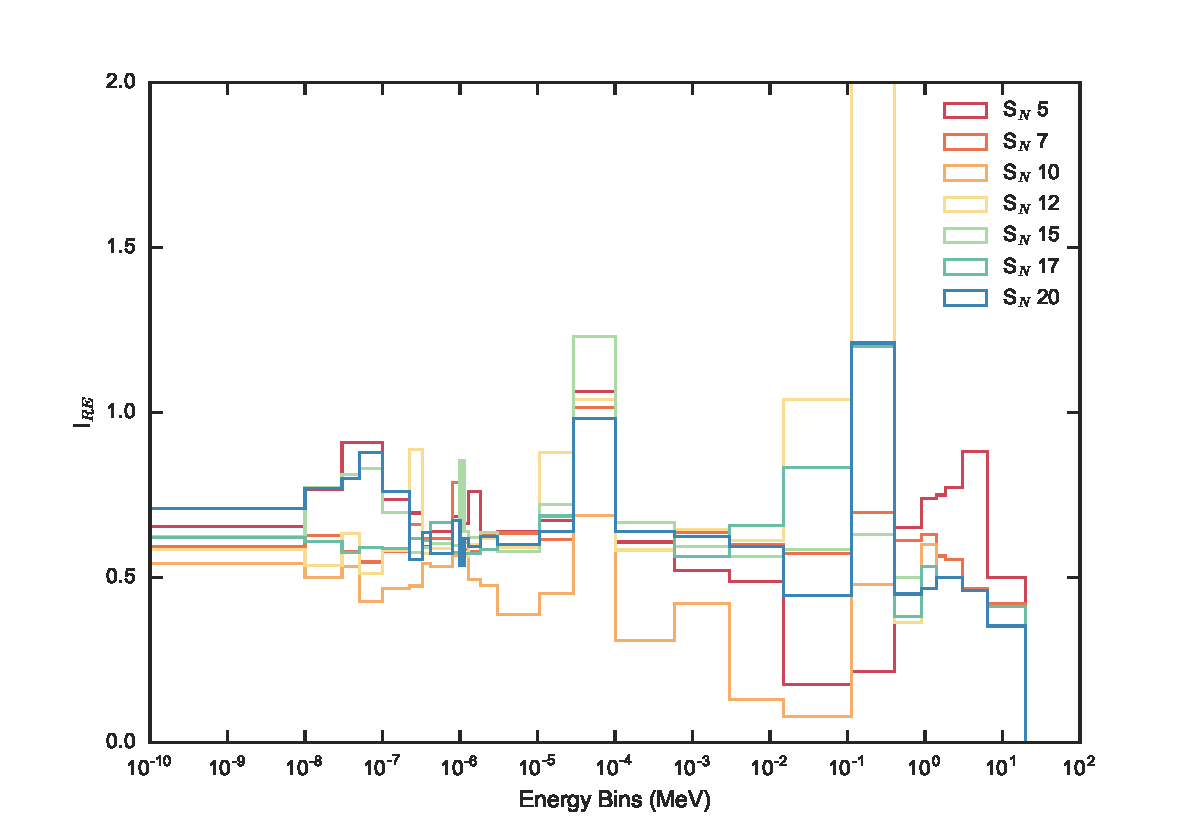
\includegraphics[height=10cm]{./chapters/characterization_probs/figures/angle/prob_1/compare_err_quad.pdf}
  \caption[Relative error improvement factor (Eq. \eqref{eq:I-RE}) between CADIS-$\Omega$ and
  CADIS as a function of quadrature order for steel beam embedded in concrete.]
  {Relative error ratio (Eq. \eqref{eq:I-RE}) between CADIS-$\Omega$ and
   CADIS as a function of quadrature order for the problem with
   a steel beam embedded in concrete.}
  \label{fig:prob_1_quad_I_RE}
\end{figure}

While Figure \ref{fig:sn_errs} shows the how the relative errors of the tally
change with different quadrature orders, we have no indication of how CADIS and
CADIS-$\Omega$ change in comparison to one another. Figure
\ref{fig:prob_1_quad_I_RE} shows the relative error improvement factor for each
quadrature order. A value below unity indicates that CADIS-$\Omega$ achieved a
better relative error than CADIS for that bin and quadrature order. In this
figure we can clearly see the effect that the problematic energy bins in each
method has on the improvement factor. In CADIS we observed that bins in the
$10^{-3}$ to $10^{-1}$ were problematic for quadrature order 10; this is
reflected in the very low value of I$_{RE}$ for that energy range and quadrature
order. Conversely, we observed that CADIS-$\Omega$ had a very problematic energy
bin between $10^{-1}$ and $10^{0}$ at quadrature order 12. The value of this
I$_{RE}$ is far above the y-limit of Figure \ref{fig:sn_errs}.

Figure \ref{fig:sn_errs} also shows that quadrature order 10 is generally order
in which CADIS-$\Omega$ outperforms CADIS the most. For this quadrature error,
CADIS-$\Omega$ achieves the lowest error when compared to CADIS. An exception to
this is observed at energy regions above ~$3^{-1}$, whre the highest quadrature
orders outperform CADIS. In the low ($<10^{-5}$) and high ($>10^{0}$),
CADIS-$\Omega$ obtains lower relative errors than CADIS for all quadrature
orders.

\begin{figure}[h!]
  \centering
  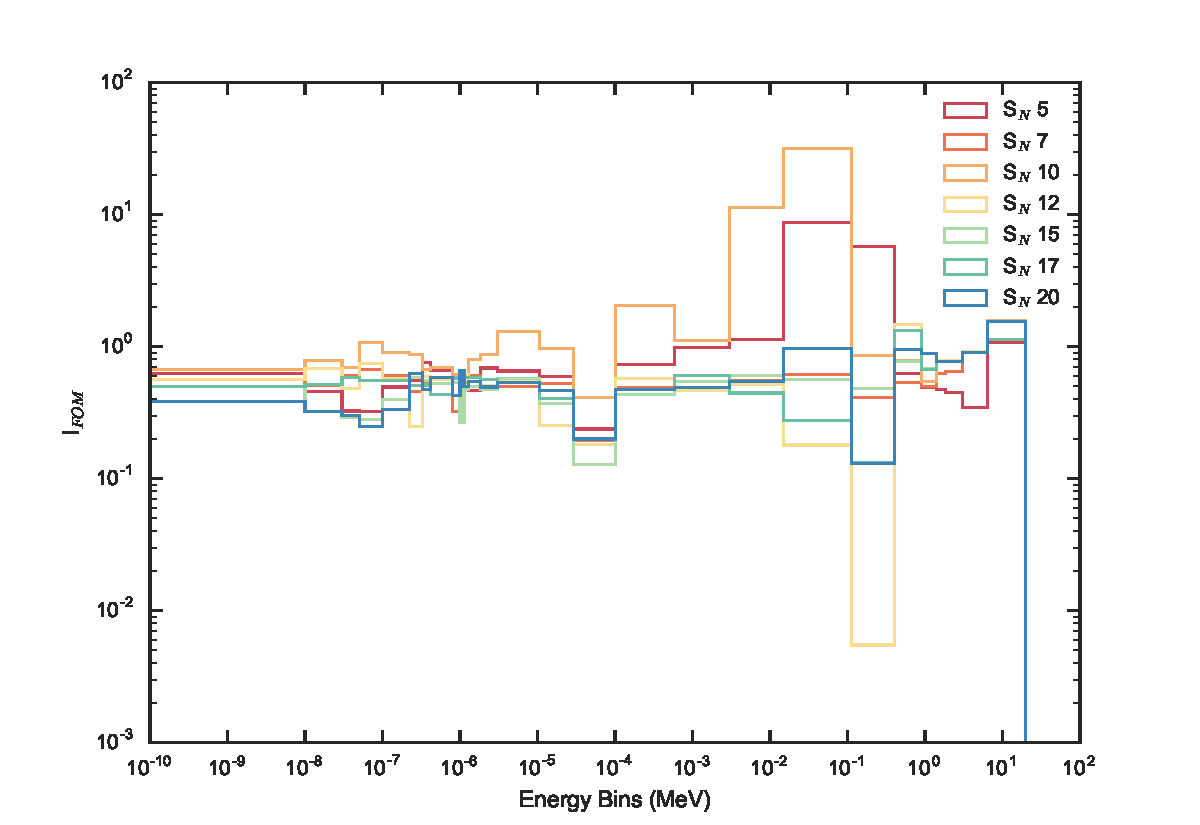
\includegraphics[height=10cm]{./chapters/characterization_probs/figures/angle/prob_1/compare_fom_quad.pdf}
  \caption[Figure of merit improvement factor  (Eq. \eqref{eq:I-FOM}) between CADIS-$\Omega$ and
  CADIS with changes in quadrature order for steel beam embedded in concrete.]
  {Figure of merit improvement factor  (Eq. \eqref{eq:I-RE}) between CADIS-$\Omega$ and
   CADIS with changes in quadrature order for the problem with
   a steel beam embedded in concrete.}
  \label{fig:prob_1_quad_I_FOM}
\end{figure}

Figure \ref{fig:prob_1_quad_I_FOM} complements the results to Figure
\ref{fig:prob_1_quad_I_RE}. Here the FOM improvement factor is plotted rather
than the relative error improvement factor. Because a higher valued FOM is a
better result, values above $10^{0}$ indicate that CADIS-$\Omega$ outperformed
CADIS. On this plot we see clearly that for higher energies there is a
larger difference between CADIS-$\Omega$ and CADIS, as observed with I$_{RE}$.

Let us return again to the high and low-energy regions of the plot, as explored
with Figure \ref{fig:prob_1_quad_I_RE}. In this region it can be observed
that for low energies, generally I$_{FOM}$ decreases with increasing
S$_{N}$ order. This behavior reverses at high energies, where the ratio
increases with increasing quadrature order. This may be an effect of anisotropy
in each energy group, as the highest energy has the most anisotropy in the flux.
Recall from Section \ref{subsec:resultsbeam} that the anisotropy metric was much
higher at high energies than it was at low energies. It is possible that for
this more anisotropic energy group, increasing the quadrature order improves the
importance map in the $\Omega$ methods more, resulting in a better relative
error. This would also explain the converse behavior at low energies. Low
energies generally have more isotropic behavior, and increasing the quadrature
order would not help to improve anisotropy information in the importance map.
As a result, increasing quadrature order would not help the FOM at low energies.

Despite a higher relative FOM at high energies, in higher quadrature orders
CADIS-$\Omega$'s performance does not generally exceed CADIS'. For quadrature
order 20, CADIS-$\Omega$'s FOM is almost always lower than CADIS. On Figure
\ref{fig:prob_1_quad_I_FOM}, the cooler toned lines which correspond to higher
quadrature orders have lower values than the warmer toned lines.
For quadrature order 5,
the relative errors on Figure \ref{fig:prob_1_quad_I_RE} were bookended by
higher order quadratures at middle and low energies. This behavior is not the
same in Figure \ref{fig:prob_1_quad_I_FOM}, where the lowest quadrature order
has a higher relative FOM than any of the quadrature orders above 10. This means
that the time required to solve higher quadrature orders affects the FOM more
negatively than the quadrature order decreases the relative error (and
positively affects the FOM).

%[Show FOMs as a function of quad order for first problem] \\
%
%[Show interesting anisotropy plots for extreme-valued quad types.] \\
%
%[Show flux maps for each extreme-valued problem in region of interest.] \\
%
%[Describe results.] \\
%
%[Show FOMs as a function of quad order for second problem] \\
%
%[Show interesting anisotropy plots for extreme-valued quad types.] \\
%
%[Show flux maps for each extreme-valued problem in region of interest.] \\
%
%[Describe results.] \\

\subsection{Scattering (P$_N$) Order}
\label{subsec:pnorder}

Table \ref{tab:pn_foms} is much like that of Table \ref{tab:quad_foms}, but with
differing P$_N$ orders than quadrature orders. The table is split into four
vertical regions, the first three corresponding to FOMS calculated with
different relative errors and the last corresponding to Monte Carlo and hybrid
runtimes for the problem. Each of the three first subsections of the table have
different trends with P$_N$ order, which will be described in the next several
paragraphs.

In the tally average relative error subsection of the table one can see that
CADIS has a dip in the FOM for P$_N$ order 3; both P$_N$ orders one and five are
higher overall. This effect is not seen in CADIS-$\Omega$, where a decrease in
the FOM is observed with increasing P$_N$ order. As a result, for
CADIS-$\Omega$, lower P$_N$ orders are sufficient for generating biasing
parameters, but for standard CADIS the highest P$_N$ order achieves the best
tally average FOM.

As with Table \ref{tab:quad_foms}, a dip in CADIS' FOMs is also observable in the
maximum relative error subsection of the table. However, this dip observable at
P$_N$ order 3 also exists in CADIS-$\Omega$. If a user desires to have all
tally bins to be below a particular relative error, P$_N$ order 3 is the worst
option for both methods in this problem. For P$_N$ order 1 CADIS-$\Omega$ is the
better choice, and for P$_N$ order 5, CADIS is the better choice.

\begin{table}[h!]
  \centering
  \begin{tabular}{lc|ccccc}
\toprule
{} & {} & \multicolumn{2}{c}{CADIS}  & \multicolumn{2}{c}{CADIS-$\Omega$}  & analog \\
{} &  P$_N$ order &     MC  &   MC$_{hybrid}$ & MC & MC$_{hybrid}$ &  MC \\
\midrule
\multirow{3}{*}{tally avg} &  P$_N$ 1 &    1.76e+03 &  1.74e+03 &   2.99e+03 &
2.96e+03 &    \multirow{3}{*}{1.39} \\
     {}    &  P$_N$ 3 &         671 &       661 &   2.97e+03 &     2.94e+03 & {} \\
     {}    &  P$_N$ 5 &    2.21e+03 &  2.16e+03 &   2.45e+03 &     2.42e+03 & {}  \\
\midrule
\multirow{3}{*}{max RE} &  P$_N$ 1 &        7.19 &      7.09 &       8.06 &
7.98 &  \multirow{3}{*}{0.0448} \\
     {}    &  P$_N$ 3 &        3.75 &       3.7 &       6.74 &         6.66 & {} \\
     {}    &  P$_N$ 5 &        14.8 &      14.5 &       8.24 &         8.12 & {} \\
\midrule
\multirow{3}{*}{min RE} &  P$_N$ 1 &     1.5e+03 &  1.48e+03 &   1.33e+03 &     1.31e+03 &      -- \\
     {}    &  P$_N$ 3 &    1.43e+03 &  1.41e+03 &   1.32e+03 &     1.31e+03 &      -- \\
     {}    &  P$_N$ 5 &    1.24e+03 &  1.22e+03 &   1.57e+03 &     1.55e+03 &      -- \\
\midrule
\multirow{3}{*}{time (mins)} &  P$_N$ 1 &         394 &       399 &   2.09e+03 &
2.11e+03 &    \multirow{3}{*}{22.3} \\
     {}    &  P$_N$ 3 &         413 &       419 &    2.1e+03 &     2.13e+03 & {}  \\
     {}    &  P$_N$ 5 &         559 &       571 &   2.55e+03 &     2.59e+03 & {} \\
\bottomrule
\end{tabular}

  \caption[Figure of Merit results for steel beam embedded in concrete, with
  variations in P$_{N}$ order.]{Figure of Merit results for steel beam embedded in concrete, with
    variations in P$_{N}$ order. Subdivisions of the table indicate
calculations of the FOM using different relative errors. The analog case has a
single value for each relative error as it is not dependent on changes in
deterministic calculation parameters.}
  \label{tab:pn_foms}
\end{table}

Next, comparing the FOMs for CADIS and CADIS-$\Omega$ using the minimum relative
errors, some interesting trends are visible. In Table \ref{tab:quad_foms} we
observed that as quadrature order increased, the minimum relative error FOM
generally increased or stayed the same for both CADIS and
CADIS-$\Omega$. This is not the case in Table \ref{tab:pn_foms}. As P$_N$ order
increases, the minimum relative error FOM for CADIS decreases, but for
CADIS-$\Omega$ it increases. This means that increasing P$_N$ order does not
move more particles (and reduce the relative error) in the energy bin with the
lowest relative error in CADIS, but it does in CADIS-$\Omega$.

Note that the FOMS using T$_{hybrid}$ do not decrease as much with increasing
P$_N$ order as they did for increasing quadrature order for CADIS-$\Omega$. As
noted previously, this is due to the lower I/O requirements for differing P$_N$
orders for CADIS-$\Omega$. As a result,
CADIS and CADIS-$\Omega$ have similar increases in computational
resources with increasing P$_N$ order.

As with Table \ref{tab:quad_foms}, Table \ref{tab:pn_foms} shows that the
behavior of the FOMs does not follow the same trends between different relative
error measurements. Depending on the user requirements for the method, one may
be a better option than the other. Looking at the timing results in the last
section of the table, we can see that CADIS-$\Omega$ takes at least five times
longer than CADIS to perform a hybrid run. This is similar to what was observed
for the quadrature order results. However, increasing P$_N$ order increased
CADIS Monte Carlo runtimes roughly 40\% between P$_N$ orders 1 and 5, and
increased CADIS-$\Omega$ runtimes about 22\% for the same quadrature orders.
While the total amount of time added to CADIS-$\Omega$ runtimes is longer, it is
relatively less than the amount that was added to CADIS.

\begin{figure}[htb!]
  \centering
  \begin{subfigure}[t]{\textwidth}
    \centering
    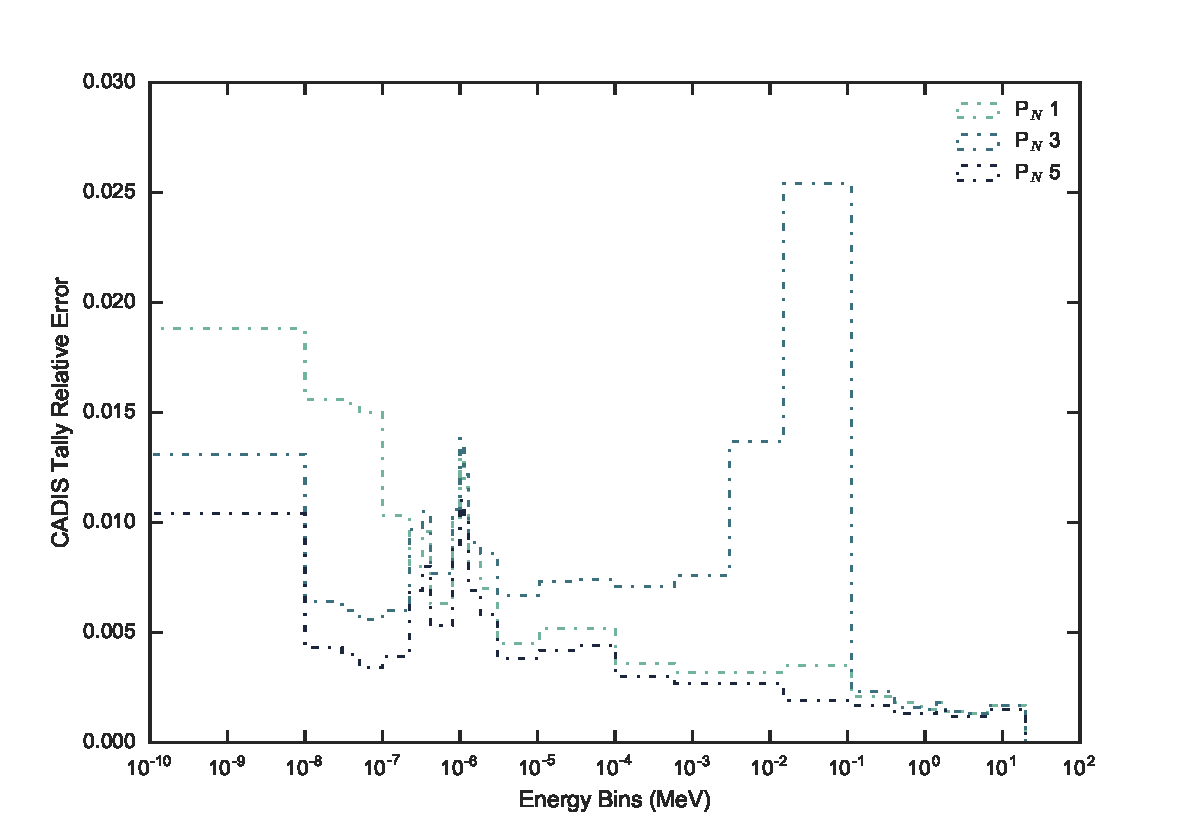
\includegraphics[width=\linewidth]{./chapters/characterization_probs/figures/angle/prob_1/err_pN_cadis.pdf}
    \caption{Relative errors of CADIS results for differing P$_N$ orders.}
    \label{fig:pn_cad_err}
  \end{subfigure}
\end{figure}
\begin{figure}[htb!]\ContinuedFloat
  \centering
  \begin{subfigure}[t]{\textwidth}
    \centering
    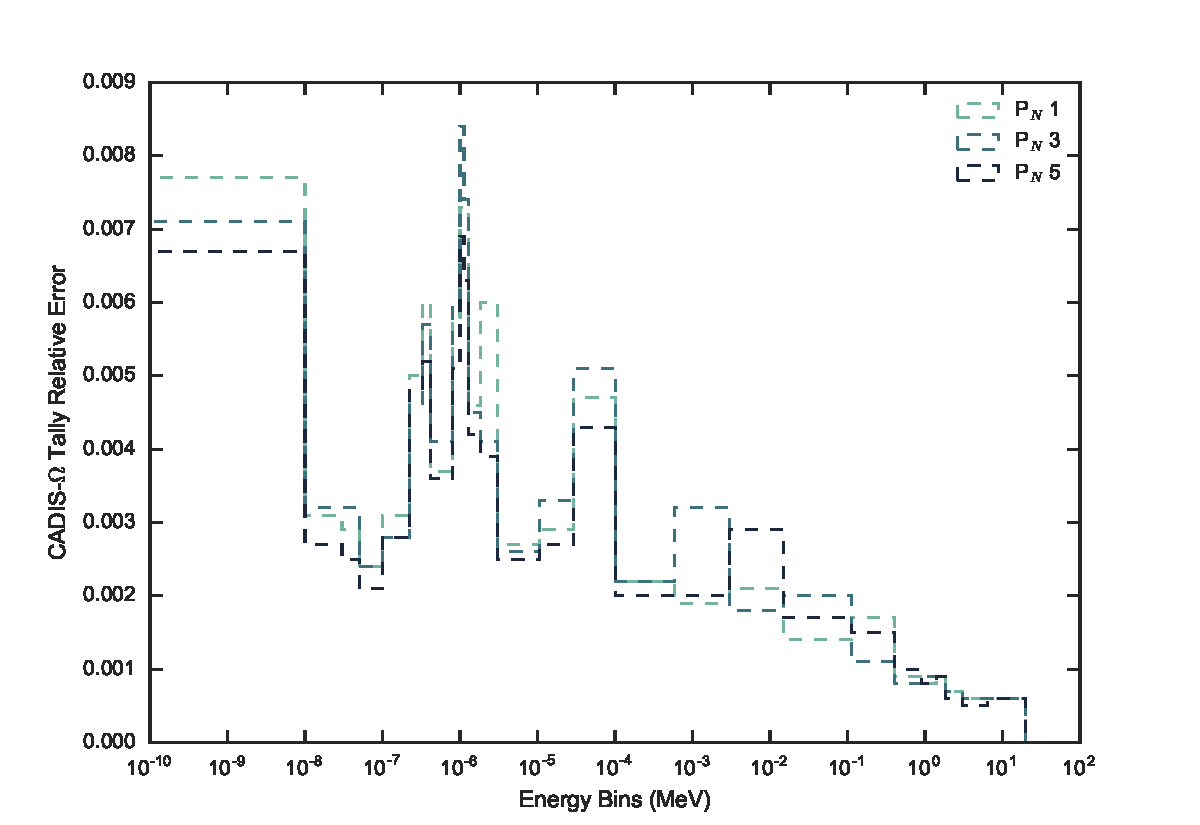
\includegraphics[width=\linewidth]{./chapters/characterization_probs/figures/angle/prob_1/err_pN_cadisangle.pdf}
    \caption{Relative errors of CADIS-$\Omega$ results for differing P$_N$
    orders.}
    \label{fig:pn_cadangle_err}
  \end{subfigure}
  \caption[Relative error results for CADIS and CADIS-$\Omega$ with changes in
  P$_N$ order for the problem with a steel beam in concrete.]
  {Relative error results for CADIS and CADIS-$\Omega$ with changes in
  P$_N$ order for the problem with a steel beam in concrete.}
  \label{fig:quad_errs}
\end{figure}

Figures \ref{fig:pn_cad_err} and \ref{fig:pn_cadangle_err} provide additional
information on interpreting Table \ref{tab:pn_foms}. Figure \ref{fig:pn_cad_err}
shows the tally relative error results for each of the P$_N$ order CADIS runs,
and Figure
\ref{fig:pn_cadangle_err} shows the same results for CADIS-$\Omega$. In Figure
\ref{fig:pn_cad_err} the highest relative error for CADIS'
P$_N$ order 1 is the most thermal energy bin, for P$_N$ order 3 is the tally bin
between $10^{-2}$, and for P$_N$ order 5 is the resonance region around
$10^{-6}$. The lowest relative error bin, however, is the same for all P$_N$
orders. This bin is located just below the highest energy bin. The shifting
location of the highest valued relative error energy bin helps to explain the
strange trend of the FOMS in the second region of Table \ref{tab:pn_foms}.
Because the relative error bins  become larger in epithermal
energy groups at P$_N$ order 3, and this shift spans several energy bins, it
also helps to explain the tally average FOM shift to a lower value at P$_N$
order 3.

In Figure \ref{fig:pn_cadangle_err}, no significant shift in the relative error
happens at P$_N$ order 3. However, we can observe a shifting location of the highest
valued relative error. At P$_N$ order 1 the highest valued relative error for
CADIS-$\Omega$ is the lowest energy bin. At P$_N$ order 3 the highest relative
error bin is the resonance region located near $10^{6}$ MeV,  and at P$_N$ order
5 these two bins appear to have a similar relative error. The highest overall
observed relative error occurs in P$_N$ order 3, which is why we see the shift
to a lower FOM at P$_N$ order 3 for the maximum relative error subsection of
Table \ref{tab:pn_foms}. This shift is not as significant as the several-bin
spanning shift in CADIS, so it does not affect the tally average FOM in
CADIS-$\Omega$.

\begin{figure}[h!]
  \centering
  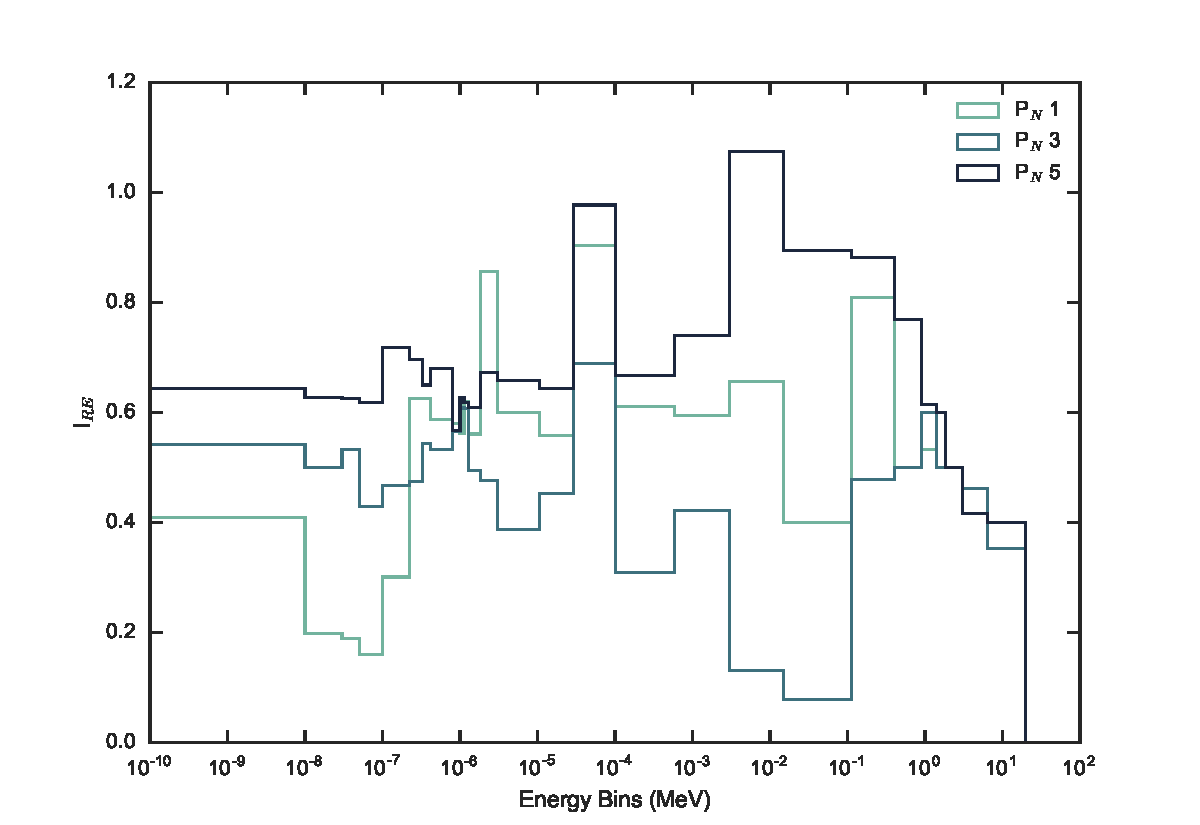
\includegraphics[height=10cm]{./chapters/characterization_probs/figures/angle/prob_1/compare_err_pN.pdf}
  \caption[Relative error improvement factor (Eq. \eqref{eq:I-RE}) between CADIS-$\Omega$ and
  CADIS with changes in P$_N$ order for steel beam embedded in concrete.]
  {Relative error improvement factor (Eq. \eqref{eq:I-RE}) between CADIS-$\Omega$ and
   CADIS with changes in P$_N$ order for the problem with a
   steel beam embedded in concrete.}
  \label{fig:prob_1_pN_I_RE}
\end{figure}

From Figures \ref{fig:pn_cadangle_err} and \ref{fig:pn_cad_err}, we can conclude
that shifts in the relative error that dramatically change between P$_N$ orders
can affect the overall tally convergence. This shift is not predictable, and may
not be observed with other

\begin{figure}[h!]
  \centering
  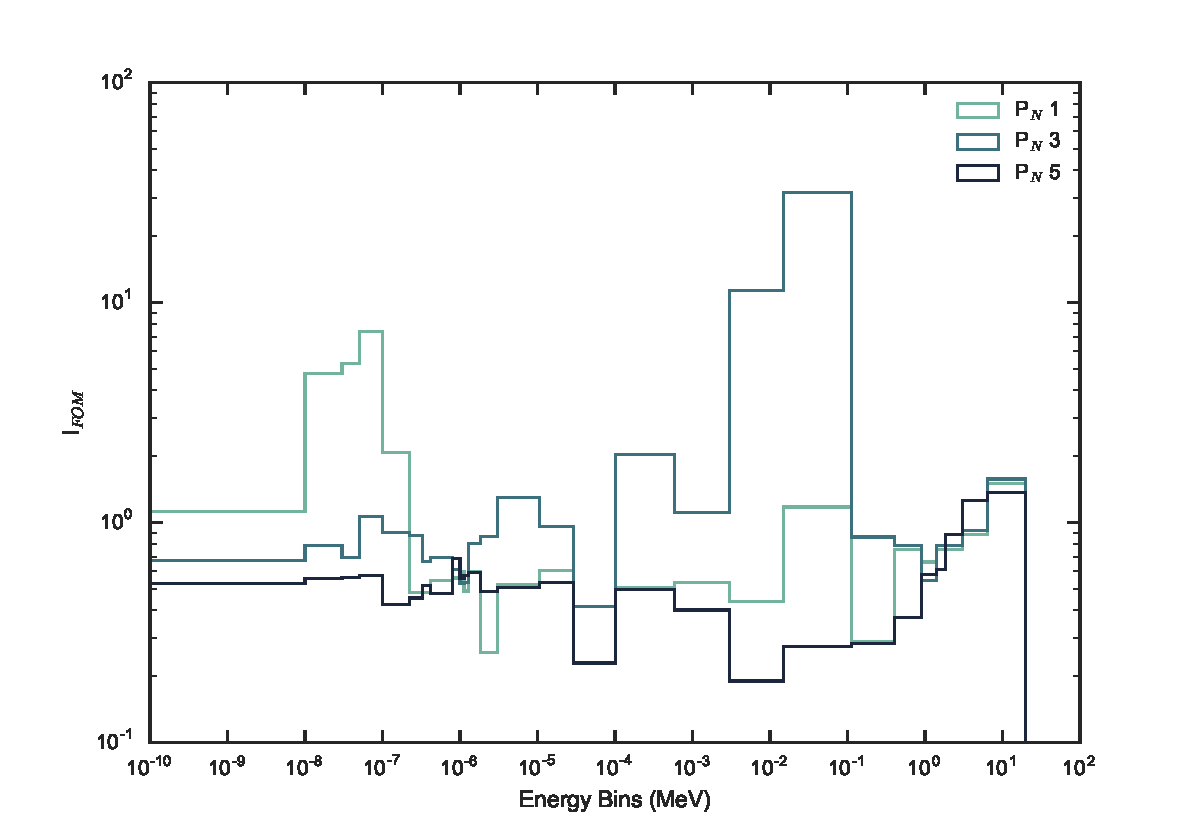
\includegraphics[height=10cm]{./chapters/characterization_probs/figures/angle/prob_1/compare_fom_pN.pdf}
  \caption[Figure of merit improvement factor (Eq. \eqref{eq:I-FOM}) between CADIS-$\Omega$ and
  CADIS as a function of P$_N$ order for steel beam embedded in concrete.]
  {Figure of merit improvement factor (Eq. \eqref{eq:I-FOM}) between CADIS-$\Omega$ and
   CADIS as a function of P$_N$ order for the problem with a
   steel beam embedded in concrete.}
  \label{fig:prob_1_pN_I_FOM}
\end{figure}

% [Show FOMs as a function of pN order for first problem] \\
%
% [Show interesting anisotropy plots for extreme-valued pN orders] \\
%
% [Show flux maps for each extreme-valued problem in region of interest.] \\
%
% [Describe results.] \\
%
% [Show FOMs as a function of pN order for second problem] \\
%
% [Show interesting anisotropy plots for extreme-valued pN orders] \\
%
% [Show flux maps for each extreme-valued problem in region of interest.] \\
%
% [Describe results.] \\

\subsection{Observations}
\label{subsec:observations}

Subsections \ref{subsec:pnorder} and \ref{subsec:quadorder} showed how varying
P$_N$ order and quadrature order changed the tally results and tally
convergences for the steel beam problem embedded in concrete. A number of
observations can be made from this study.

Figures \ref{fig:angle_err_improvements} and \ref{fig:angle_fom_improvements}
summarize the data from the previous subsection. In Figure
\ref{fig:angle_err_improvements}, the ratio of the relative error in each tally
bin is taken between the lowest and highest-valued parameter run of the
parametric study. For P$_N$ order (the purple lines in the figure)
this would be $RE_{P_N 1}/RE_{P_N 5}$ and for
quadrature order (the green lines in the figure) it would be $RE_{S_N 5}/
RE_{S_N 20}$. A high ratio means that the relative error decreased more for
the higher-valued parameter (P$_N$ order 5 or S$_N$ order 20).

\begin{figure}[h!]
  \centering
  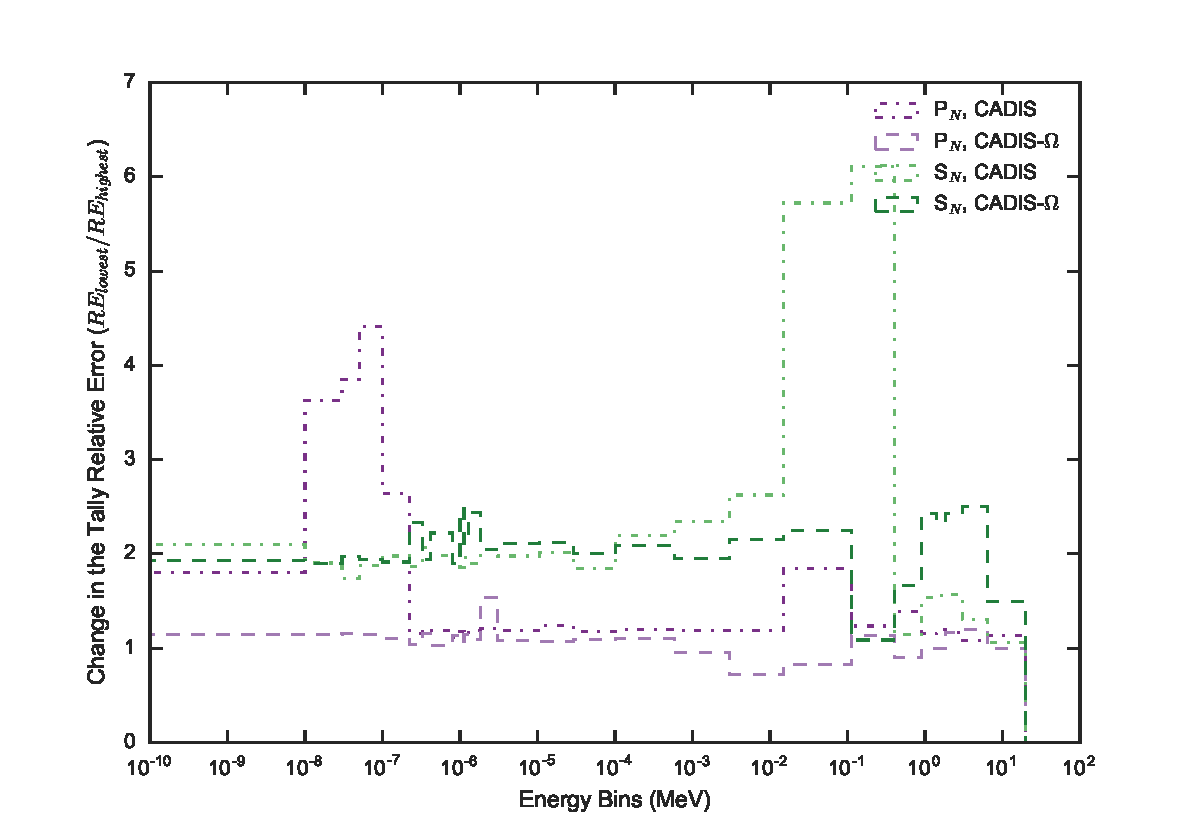
\includegraphics[height=10cm]{./chapters/characterization_probs/figures/angle/prob_1/improvement_err_allmethds.pdf}
  \caption[Ratio in the relative errors between the lowest and highest variable in the angle
  sensitivity study for CADIS and CADIS-$\Omega$.]{Ratio in the relative errors between
    the lowest and highest variable in the angle sensitivity study for CADIS and CADIS-$\Omega$.}
  \label{fig:angle_err_improvements}
\end{figure}

In

\begin{figure}[h!]
  \centering
  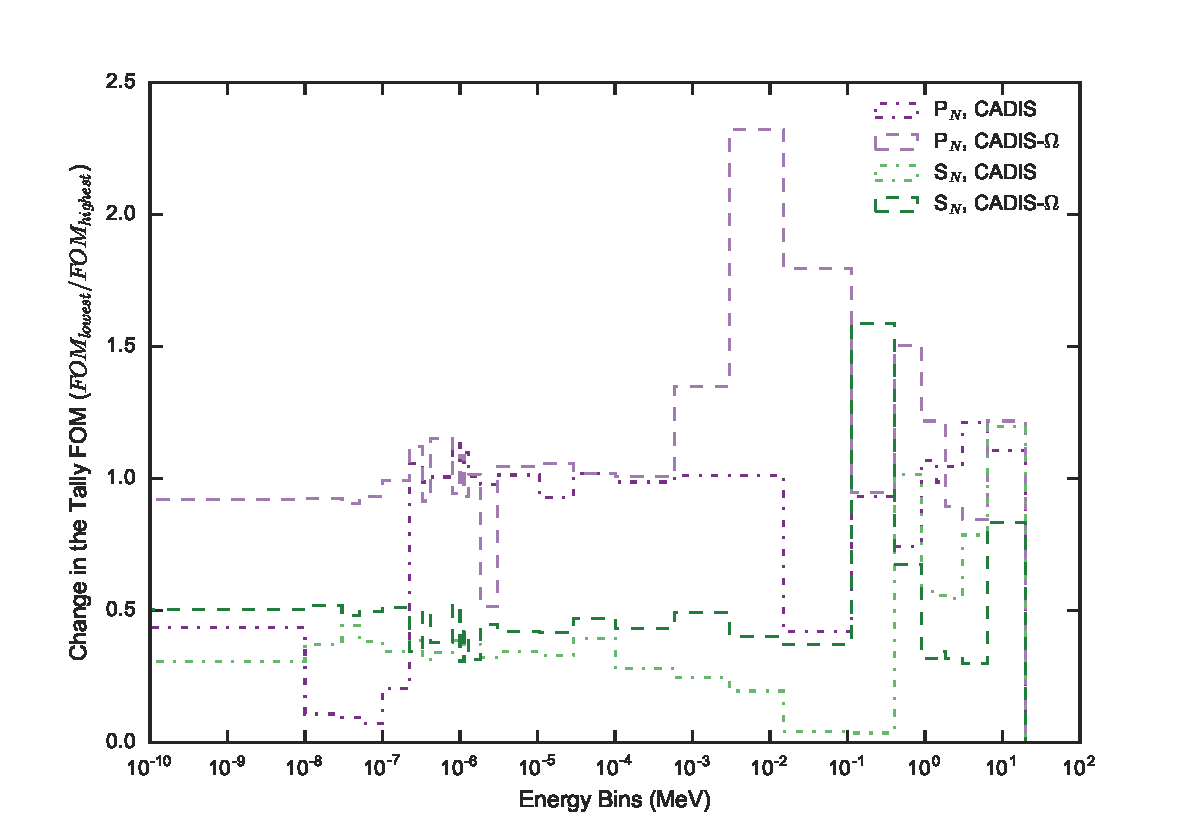
\includegraphics[height=10cm]{./chapters/characterization_probs/figures/angle/prob_1/improvement_fom_allmethds.pdf}
  \caption[Ratio in the figure of merits between the lowest and highest variable in the angle
  sensitivity study for CADIS and CADIS-$\Omega$.]{Ratio in the figure of merits between
    the lowest and highest variable in the angle sensitivity study for CADIS and CADIS-$\Omega$.}
  \label{fig:angle_fom_improvements}
\end{figure}

[Go back through results and highlight benefits and pitfalls.] \\

[Describe reasons why these might have occurred. Follow up with a list of options
that could be done in further testing to confirm reasons.] \\

It should also be noted that while the angle-dependent parametric study revealed
how P$_N$ order and quadrature order may affect a problem's convergence, it is
by no means a universially prescriptive approach. Section \ref{sec:CharResults}
showed how different the characterization problems' results were, depending on
the source definition, the material composition of the problem, and the
geometric configuration of the problem. Using the deterministic parameter
choices that appear the best for the steel beam in concrete may not be the best
for, say, a multi-turn labyrinth. This will be an important aspect of future
work.
